\section*{Exercice 1?? -- Train épicycloïdal}

\setcounter{exo}{0}

Soit le train épicycloïdal suivant. 

\begin{center}
 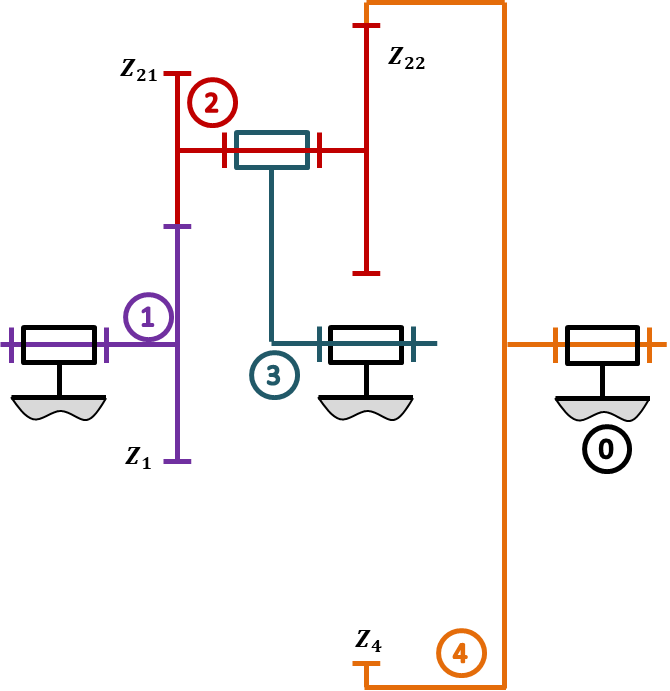
\includegraphics[width=.6\linewidth]{054_01}
\end{center}
\fi




\subparagraph{}
\textit{Déterminer $\omega_{40}$ en fonction de  $\omega_{30}$ et $\omega_{10}$.}
 \ifprof
 \begin{corrige}
 
 En bloquant le porte satellite, on a : $\dfrac{\omega_{43}}{\omega_{13}}=-\dfrac{Z_{1}Z_{22}}{Z_{21}Z_{4}}$.
  On a donc, 
  $\dfrac{\omega_{40}+\omega_{03}}{\omega_{10}+\omega_{03}}=-\dfrac{Z_{1}Z_{22}}{Z_{21}Z_{4}}$

  $\Leftrightarrow \omega_{40}+\omega_{03}=-\dfrac{Z_{1}Z_{22}}{Z_{21}Z_{4}}\left( \omega_{10}+\omega_{03} \right)$
  
  $\Leftrightarrow \omega_{40}=-\dfrac{Z_{1}Z_{22}}{Z_{21}Z_{4}}\left( \omega_{10}+\omega_{03} \right)-\omega_{03}$
  
    $\Leftrightarrow \omega_{40}=-\dfrac{Z_{1}Z_{22}}{Z_{21}Z_{4}}\left( \omega_{10}+\omega_{03} \right)+\omega_{30}$
    
      $\Leftrightarrow \omega_{40}=-\dfrac{Z_{1}Z_{22}}{Z_{21}Z_{4}}\omega_{10}+\omega_{30}\left( 1+\dfrac{Z_{1}Z_{22}}{Z_{21}Z_{4}} \right)$

 \end{corrige}
 \else
 \fi




\subparagraph{}
\textit{On suppose que $\omega_{40}$ est bloqué. Exprimer le rapport $\dfrac{\omega_{30}}{\omega_{10}}$.}
\ifprof
 \begin{corrige}
$0=-\dfrac{Z_{1}Z_{22}}{Z_{21}Z_{4}}\omega_{10}+\omega_{30}\left( 1+\dfrac{Z_{1}Z_{22}}{Z_{21}Z_{4}} \right)$

$\Leftrightarrow \dfrac{Z_{1}Z_{22}}{Z_{21}Z_{4}}\omega_{10}=\omega_{30}\left( 1+\dfrac{Z_{1}Z_{22}}{Z_{21}Z_{4}} \right)$


$\Leftrightarrow \dfrac{\omega_{30}}{\omega_{10}} 
= \dfrac{\dfrac{Z_{1}Z_{22}}{Z_{21}Z_{4}}}{ 1+\dfrac{Z_{1}Z_{22}}{Z_{21}Z_{4}} }
= \dfrac{Z_{1}Z_{22}}{ Z_{21}Z_{4}+Z_{1}Z_{22} }$


 \end{corrige}
 \else
 \fi